% Created 2013-03-24 Sun 22:53
\documentclass[a4paper,11pt]{article}
\usepackage[utf8]{inputenc}
\usepackage[T1]{fontenc}
\usepackage{fixltx2e}
\usepackage{graphicx}
\usepackage{longtable}
\usepackage{float}
\usepackage{wrapfig}
\usepackage{soul}
\usepackage{textcomp}
\usepackage{marvosym}
\usepackage{wasysym}
\usepackage{latexsym}
\usepackage{amssymb}
\usepackage{hyperref}
\tolerance=1000
\usepackage{fontspec}
\usepackage[titletoc,page,title]{appendix}
\usepackage{biblatex}
\usepackage{metalogo}
\usepackage{graphicx}
\usepackage{moreverb}
\usepackage{subfig}
\let\iint\relax % otherwise errors are thrown by amsmath. Defined in latexsym
\let\iiint\relax
\usepackage{amsmath}
\usepackage{hyperref}
\usepackage{tikz}
\usetikzlibrary{positioning}
\bibliography{fyp}
\defaultfontfeatures{Mapping=tex-text}
\setromanfont[Ligatures={Common},Numbers={Lining}]{Linux Libertine}
\providecommand{\alert}[1]{\textbf{#1}}

\title{Time Delay Estimation in Gravitationally Lensed Photon Stream Pairs}
\author{\Large{Micha{\l} Staniaszek} \\\small{Supervisor: Peter Ti{\v{n}}o}}
\date{\today}
\hypersetup{
  pdfkeywords={},
  pdfsubject={},
  pdfcreator={Emacs Org-mode version 7.8.11}}

\begin{document}

\maketitle


\thispagestyle{empty}
\newpage
\pagenumbering{roman}
\begin{abstract}
In this report, we present a system for estimating the time delay $\Delta$
between multiple realisations of a Poisson process with the underlying function
$\lambda(t)$, with particular application to gravitationally lensed photon
streams. We develop a linear estimator based on weighted least squares, and a
kernel density estimator which we use to estimate $\lambda(t)$. We then
introduce two methods for estimating the value of $\Delta$ using the function
estimates, one using inter-function area, and another using probability density
functions. Finally, we compare the performance of the two function estimation
methods and time delay estimation methods on simulated data, and show that there
is not a significant difference between the approaches.

\vspace{1.0cm}\textbf{Keywords: }Poisson process, gravitational lensing,
 machine learning, linear estimation

\begin{center}
\vspace*{\fill}\scriptsize{Typeset in Linux Libertine using \XeLaTeX}.
\end{center}
\end{abstract}
\newpage
\tableofcontents
\newpage
\pagenumbering{arabic}
\section{Introduction}
\label{sec-1}

With continued advances in computing and sensing technologies, the amount of
data that can be gathered from both everyday objects and scientific experiments
has increased rapidly. However, more data is not always a blessing---it must be
stored and analysed for it to have any use, and this is not an easy task when
one has terabytes of data to deal with. The Large Hadron Collider at CERN is one
perhaps extreme example, producing on the order of five terabytes of data each
second. Storing this amount of data, let along analysing it is impossible, and
so multiple stages of intelligent filtering are applied, reducing the throughput
to 100 gigabytes per second, and then further to around 200 megabytes per
second, where it is finally stored, producing almost two CDs each second
\cite{WLCGproc}. This project focuses on creating the foundations for a system
to do such intelligent filtering, but in the context of astronomical data. The
volume of data produced by modern telescopes, while not on the same scale as the
LHC, is nonetheless overwhelming. Image sizes of one to two gigabytes are not
uncommon, and deciding what data is actually relevant is not a trivial task
\cite{starck2002handbook}. Using intelligent filtering algorithms, it should be
possible to flag up interesting-looking data for further study. While there are
many areas in which such capabilities would be useful, we are particularly
interested in finding candidates for images of gravitationally lensed
objects. In order to do this, it is necessary to find pairs of observations of
photon flux which appear to have the same underlying function. More precisely,
given a set of data containing the time of arrival of photons from a particular
source, henceforth called a \emph{stream}, we wish to find another stream which,
when shifted in time by some value $\Delta$, has similar numbers of photons
arriving in a given interval as the first stream. We call $\Delta$ the
\emph{delay} between the two streams. In this project, we develop a system which
can generate simulated photon streams using Poisson processes, use linear
regression to estimate the underlying function of a given stream, and, given the
function estimates of two streams, estimate the time delay between them. Knowing
the value of the time delay has many applications in astrophysics, and with more
precise estimates, more accurate calculations can be made to increase our
understanding of the universe we live in.

\begin{itemize}
\item strong lensing has delays on the order of hundreds of days, but weak lensing
  is more like on the order of hours - no longer sufficient to calculate flux
  for a single day, must do it in a different way, by measuring individual
  photon arrival times.
\end{itemize}

In section \ref{sec-2} we discuss the concepts underpinning the project in more
detail, with a more in-depth explanation of the issues surrounding the
calculation of the time delay and its uses. In section \ref{sec-3} we introduce our method of generating photon streams from Poisson
processes. Section \ref{sec-2-3} shows our approach to estimating the
underlying function of a given stream of photons. Our methods of calculating the
time delays between multiple photon streams are explained in section \ref{sec-5}. Section \ref{sec-6} gives detailed information on the design and
development of the system, including the software and project management
aspects. Finally, in section \ref{sec-7} we present experimental data from both
simulated and real data and discuss the relative effectiveness of our methods.
\section{Background}
\label{sec-2}
\subsection{Gravitational Lensing}
\label{sec-2-1}

In an eight-year period starting in 1907 and ending in 1915 with the publication
of a paper on field equations of gravitation \cite{einstein1915general}, Albert
Einstein wrote many papers developing a new theory of gravitation, his general
theory of relativity. This generalisation of special relativity and Newton's law
of universal gravitation led to a revolution in the field of physics, and
remains one of the most important scientific discoveries to date. The theory
describes how spacetime is affected by the presence of matter and radiation, and
this idea has many important consequences, but one of the effects in particular
is important in the context of this report.

According to the theory, objects with mass, or massive objects, cause spacetime
to curve around them. A simple way to visualise this effect is to imagine
dropping a ball onto a sheet of cloth which has been pulled taut. The ball will
eventually come to a stop in the centre of the cloth, and cause it to sag. Here,
the sheet represents spacetime, and the ball represents anything from planets,
to stars, or even entire galaxies. Depending on the weight of the ball, the
shape of the cloth will be affected to different degrees---a ping pong ball will
have hardly any effect at all, but if we drop a bowling ball onto the sheet, the
effect will be significant. In a similar way, the amount that spacetime curves
around a massive object depends on its mass. An object with high mass will cause
a large amount of curvature, whereas a lower mass object will cause less. If a
second ball, lighter than the first, is introduced to the system, what happens?
With no initial velocity, it will roll in a straight line towards the first ball
sitting at the centre of the sheet. This is one way of thinking about gravity
and its relationship with spacetime---an object's gravitational attraction is a
result of its mass curving spacetime, and the strength of the attraction is
proportional to the mass. While objects with no mass, such as photons, cannot be
affected by gravity directly, they \emph{are} affected by the curvature of
spacetime. This bending of light rays is known as
\emph{gravitational lensing}.

The first person to study the effects of gravitational lensing was Orest
Chvolson, publishing a short note to \emph{Astronomische Nachrichten} in 1924
\cite{chwolsonlensing}. However, the concept was largely unknown until a short
calculation by Einstein was published in \emph{Science} in 1936
\cite{einsteinlensing}. Interestingly, Chvolson's note appears directly above a
note from Einstein\cite{einsteinchwolson}, but there appears to be no evidence that Einstein had ever
seen it \cite{renn2000eclipses}. The first gravitationally
lensed object to be identified was the twin quasar SBS 0957+561, in 1979, and
since then, over a hundred such objects have been discovered
\cite{firstlens,gravlenscount}. The effect of gravitational lensing is, as the
name suggests, similar to that of a lens, such as that of a camera. Unlike a
camera lens, however, gravitational lenses do not have a focal point, but
instead a focal line, resulting in images such as that shown in Figure
\ref{fig:einring} if the source (the object being lensed), the lensing object
(the massive object around which the light is being bent) and the observer lie on a
straight line. This effect is relatively rare, however, and in general rather
than a ring, multiple images of the source can be observed. In these so called
\emph{strong} lensing effects, the distortion is very clearly visible. However,
two other classes of lensing exist---\emph{weak lensing} and
\emph{microlensing}.  The effects of weak lensing cannot easily be observed
visually, but statistical techniques can show the distortion
produced. Microlensing works on even smaller scales than the other two classes,
and can be used to detect planets and stars. It has also been proposed as a
method to find objects such as black holes and brown dwarfs, which are otherwise
difficult to detect \cite{schneider2006gravitational}.
\begin{figure}
\centering
\subfloat[An Einstein ring]{
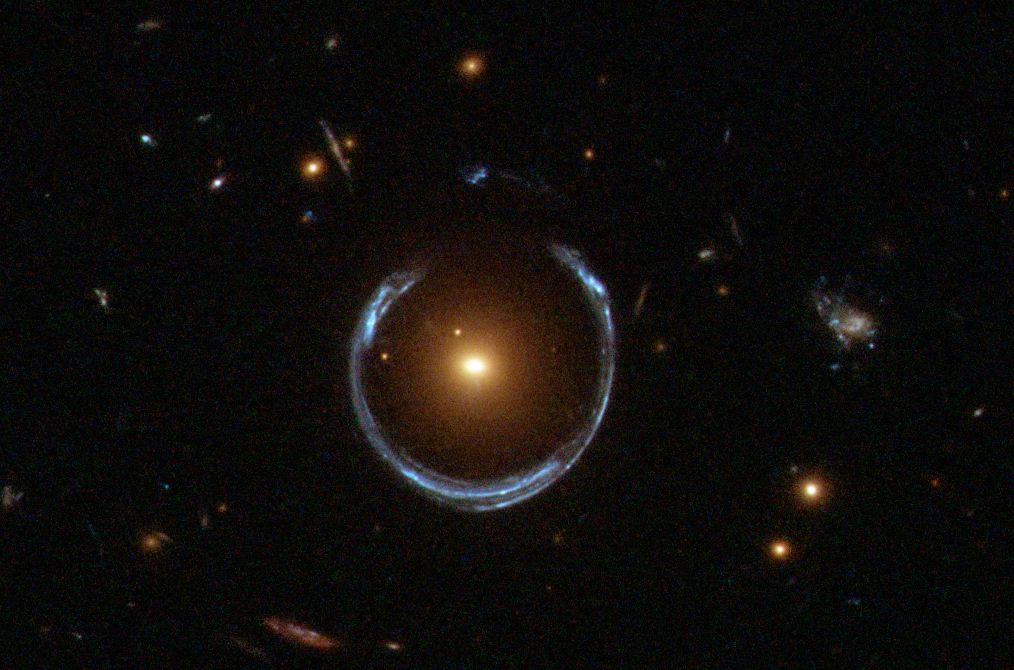
\includegraphics[width=0.4\textwidth]{einstein_ring}
\label{fig:einring}
}
\qquad
\subfloat[Einstein's cross]{
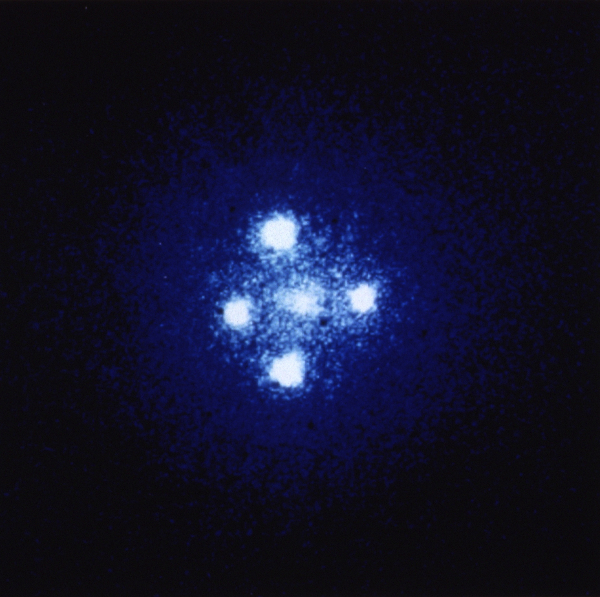
\includegraphics[width=0.4\textwidth]{einstein_cross}
\label{fig:einsteincross}
}
\caption{Two examples of strong lensing effects. a) shows light from
a distant blue galaxy being distorted by the central galaxy LRG 3-757
\cite{einsteinring}. b) shows four images of a distant quasar being lensed by a
foreground galaxy \cite{eincross}.}
\label{fig:stronglens}
\end{figure}
\subsubsection{Importance of the Time Delay}
\label{sec-2-1-1}

In gravitationally lensed systems, there is a delay between photon streams
coming from images of the source due to the bending of light. Light from one
source may have had to travel a slightly longer distance than that from the
other, and while photons travel extremely fast, over astronomical distances the
delay can become quite large. 
\begin{itemize}
\item strong lensing p86
\item Talk generally about the problem of time delay estimation
\item refer to physics papers attempting to make estimates of the delay
\item talk about time delay estimation in particular, refer to kundic et al, many others
\item talk about how better estimates benefit the scientific community
\item refer to peter's paper about the efficacy of kernel regression
\item better estimators are necessary to increase the accuracy of estimates
\item this is an experiment to see whether this method has any use
\item build on technique introduced in massey et al
\end{itemize}
\subsection{Poisson Processes}
\label{sec-2-2}

In certain situations, there are many benefits of having good models of the
numbers of events that occur in a given period. For example, being able to
estimate the number of incoming requests to a server, the number of calls made
to emergency services, and the rate of radioactive decay at any given time are
all useful in different applications. Poisson processes are \emph{stochastic
processes} that can be used to do just that. A stochastic process is a way of
representing the evolution of a random value or system over time by using
collections of random variables. Most such processes do not evolve in a
\emph{deterministic} way. That is, the way they change as time passes is not
predictable.

A Poisson process is one such process which counts the number of events and the
time at which they occur in a given time interval, and have been used to model
all of the above examples
\cite{hajjam2008approach,cannizzaro1978results,arlitt1997internet}. In their
basic form, Poisson processes have the following important properties
\cite{ross1997simulation}:
\begin{enumerate}
\item $N(0)=0$.
\begin{itemize}
\item $N(t)$ represents the total number of events that occurred up until time
     $t$. Thus, if $N(0)=0$, it follows that the process begins at $t=0$.
\end{itemize}
\item The numbers of events occurring in disjoint time intervals are independent.
\begin{itemize}
\item The \emph{independent increment} assumption. This states that $N(t)$, the
     number of events that occur up to time $t$ is \emph{independent} of the
     number $N(t+s)-N(t)$, i.e. the number of events in the time interval
     between $t$ and $s$. In other words, the number of events that occur in one
     interval does not have an effect on the number of events in any other time
     interval.
\end{itemize}
\item The probability distribution of the number of events that occur in a given
   interval is dependent only on the length of the interval.
\begin{itemize}
\item The \emph{stationary increment} assumption. The implication of this is that
     the probability distribution of $N(t+s)-N(t)$ is the same for all values of
     $t$. That is, the likelihood of a number of events $n$ occurring in the
     above time interval does not change, regardless of the value of $t$.
\end{itemize}
\item No counted occurrences are simultaneous.
\begin{itemize}
\item For all events that occur in the duration of the process, no two events
     will occur at the same time.
\end{itemize}
\end{enumerate}

The most important thing about Poisson processes is the \emph{rate parameter},
$\lambda$. This value represents the number of events that occur in each time
interval. As we are counting events, it is clear that the rate parameter can
never go below zero---there cannot be a negative number of occurrences in a
given time interval. There are two types of Poisson processes,
\emph{homogeneous} and \emph{non-homogeneous}. In a homogeneous Poisson process (HPP),
the rate parameter is constant throughout the running of the process. This means
that in every interval, the same number of events are likely to occur. In
contrast, a non-homogeneous Poisson process (NHPP) has a rate parameter which
varies. This means that the rate at which events occur varies during the running
time of the process.
\subsection{Function Estimation}
\label{sec-2-3}
\subsubsection{Linear Regression}
\label{sec-2-3-1}

Linear regression is a statistical technique used to fit lines or curves to data
points in order to find some sort of relationship between them. The number of
variables in the data is important. One of the variables is called a \emph{dependent}
variable. We want to find the relationship between this variable and the other
variables, called \emph{independent} variables. What makes one variable
dependent and another independent? Consider the expression $y=f(x)$. If $f(x)$
is some function of the variable $x$, then we know that the value of $y$ depends
on the value of $x$. This is where the names come from. In this simple example,
$x$ is the independent variable, and $y$ is the dependent variable. There can be
multiple independent variables.

Linear regression is used in many different fields to find the trend between
variables. It is heavily used in economics to make predictions about what
happens in many economical situations. Finding trends in data is useful to many
people in different ways.
\subsubsection{Kernel Density Estimation}
\label{sec-2-3-2}

This is another method which can be used to estimate functions, but which
applies specifically to the probability density function of random
variables. This technique uses \emph{kernels} to estimate the function
densities. A kernel is a function which has some parameters. To estimate
functions, kernels are centred at certain points along the axis which is being
estimated. The spread can be either at uniform intervals, each sample value,
etc. Kernels may have a weight assigned to them. Varying the parameters of
the kernels results in different properties of the estimate. There are many
different kernels that can be used. Different kernels are used in different
applications.
\begin{itemize}
\item Show some examples of different kernels
\end{itemize}
\section{Simulation of Photon Streams}
\label{sec-3}

The first step in building the system was the development of a photon stream
simulator. The ability to simulate photon streams means that the system can be
tested on many different stream types, so that we are able to determine where
its strengths and weaknesses lie. While many simulation tools are very complex,
our system does not require simulation of the source objects or the movement of
photons, as we are only interested in their arrival time. A source can be
represented by some random variable $X$, which indicates the variability of the
source with time. Different types of sources will have different types of
characteristic functions---the variation in a quasar will be very different to
that of an individual star, for example. A NHPP is an ideal way to represent
this type of system. The function $\lambda(t)$ will represent the random
variable, and the values output from the process will represent the arrival
times of the photons. $\lambda(t)$ describes the variability of the source in
time. In other words, it provides a rate parameter at each time $t$ for the
duration of the simulation. To be able to simulate a wide variety of functions,
it is necessary to have the capacity to generate functions with different
characteristics.
\subsection{Function Generation}
\label{sec-3-1}

To evaluate the performance of the function and time delay estimators, it will
be necessary to test the accuracy of the estimates on different types of
functions. To this end, the capability of generating random functions will be
very useful. To generate random functions, we make use of \large{Gaussian
kernels or just Gaussians?}. The generation process involves four simple steps:
\begin{enumerate}
\item Pick some value $\Delta t$ which represents the distance between the mean
   $\mu$ of successive Gaussians.
\item Define some value $\alpha$, where the standard deviation $\sigma$ of each
   Gaussian is determined by $\alpha\cdot\Delta t$.
\item For each Gaussian, choose some weight $w_i$, from a uniform distribution
   between -1 and 1.
\item Using some step $s$, sum all the Gaussians at each point on the $x$-axis which
   we get from these $s$ values.
\end{enumerate}

The first step defines how spread out the Gaussians should be in the interval
$[t_0, T]$ in which the function is to be generated. If the spread is large,
then depending on the standard deviation of the Gaussians there will be many
points on the interval where the value of the function is zero. On the other
hand, with a low value of $\Delta t$, most points on the line should have some
non-zero value.

The $\alpha$ parameter determines the standard deviation $\sigma$ of all the Gaussians
used to generate the function. The value of $\sigma$ is the one that affects the
final function the most. Low values will result in each Gaussian covering only a
small interval, so if the Gaussians are sufficiently spread out, the variation
in the function will be much larger than if higher values of $\sigma$ are used.

With just the above two steps, the functions generated would be very
homogeneous, because each Gaussian has the same weight. With uniform Gaussians,
there would be hills at each point where a Gaussian is centred, and very little
to speak of in between, and the height of the function would never exceed a
certain value. To introduce more variation, a weight $w_i$ is sampled uniformly
from ($w_i \sim U(-1,1)$). Uniform sampling simply means that each value between
-1 and 1 has an equal probability of being chosen. To further increase the
variation in the functions that can be generated, some multiplier can be used,
which scales the values of the weights, meaning that the function will have
larger values over the whole interval.

The final step is to calculate the values which will make up the
function. Starting at the beginning of the interval $t_0$, we sum the values of
all the Gaussians at points along the line until the end of the interval $T$ is
reached. The points that are sampled are defined by $t_i=t_{i-1}+s$, where $s$
is some sample step. The use of smaller sample steps results in a higher
resolution. The sum of the Gaussians at time $t$ can be calculated by
\begin{align}
f(t) = \sum_{g\in G}w_g\cdot e^{-(t-\mu_g)^2/2\sigma_g^2}
\end{align}
Where $G$ is the set of Gaussians which make up the function, and $w_g$, $\mu_g$
and $\sigma_g$ are the weight, mean and standard deviation respectively of the
current Gaussian being processed.

\begin{itemize}
\item random functions using gaussian sums
\item explain how the gaussians are placed, how the standard deviation is
   calculated, what effect this has on the function shape
   ($\sigma=\alpha\cdot\Delta t$)
\item examples at various alpha and delta t values?
\item $w_t\cdot e^\frac{{x-\mu}^2}{2\sigma^2}$
\end{itemize}

In addition to the random function generation, it may sometimes be useful to
generate a function from a known expression, and the system includes this
functionality as well, which will be described below.
\subsection{Generating Streams from Functions}
\label{sec-3-2}

   Once the function has been generated, we can use it to generate values for
   the random variable $X$ which governs a NHPP. To generate a NHPP, it is
   necessary to build on the generation of a HPP. It is well known that
   probability of an event occurring follows an exponential distribution. The
   rate parameter $\lambda$ determines how many events occur in a given time
   interval. Knowing this, we can calculate the time of the next event by
   sampling from this distribution. Generate a random value $U\sim U(0,1)$. The
   time $t$ to the next event is defined by
   \begin{align}\label{eq:homlambda}
   t=\frac{1}{\lambda}\log(U)
   \end{align}
   Using this calculation, it is possible to generate a realisation of a HPP for
   any length of time. This provides a base which can be extended to generate
   events from NHPPs. To generate events from the NHPP, we use a technique
   called thinning. The basic concept behind thinning is to generate a large
   amount of values, and then remove them based on some method. In the case of
   the NHPP, we generate events with a rate parameter $\lambda$, where
   $\lambda>\lambda(t)$ for $0<=t<=T$. In other words, the homogeneous lambda
   value must be larger than the value of the function we are generating from at
   any point. First, two random values are independently sampled from a uniform
   distribution between 0 and 1, $U_1,U_2\sim U(0,1)$. $U_1$ is used in
   \eqref{eq:homlambda} to find the next event time from the homogeneous process
   governed by $\lambda$. Using the time $t$ generated from that, the value of
   $\lambda(t)$ is found. Depending on the ratio between $\lambda(t)$ and
   $\lambda$, the event is kept or discarded. When the value of $\lambda(t)$ is
   close to that of $\lambda$, more events are kept because
   $U_2\leq\frac{\lambda(t)}{\lambda}$ will be true more of the time. The
   variation of $\lambda(t)$ in time means that events are generated
   proportional to the value of lambda.

\begin{itemize}
\item Need to generate event times - use Poisson process
\item start with homogeneous
\item extend homogeneous to non-homogeneous (explain math)
\item Issues with the implementation - must have $\lambda>\lambda(t)$ for all
  $0<=t<=T$.
\item Diagram showing HPP and NHPP
\item \href{http://preshing.com/20111007/how-to-generate-random-timings-for-a-poisson-process}{http://preshing.com/20111007/how-to-generate-random-timings-for-a-poisson-process}
\end{itemize}
\subsection{Implementation}
\label{sec-3-3}

    The implementation of the random and expression based function generators
    form the first part of the \emph{generator} sub-system. This part of the
    system deals with the generation of functions, and the generation of photon
    streams from these functions.
\begin{itemize}
\item gaussians as structs
\item gauss vector structs
\item functions into math library
\item separation of functions so that they can be called externally and internally
\item what can be generated
\item How expr and gauss version differ
\end{itemize}
\subsubsection{Generating from Expressions}
\label{sec-3-3-1}

\begin{itemize}
\item muparser
\item enter expression and define variables in parameter file
\item parsed in and calculated automatically
\end{itemize}
\subsubsection{Generating from Random Functions}
\label{sec-3-3-2}

\begin{itemize}
\item 
\end{itemize}
\section{Function Estimation}
\label{sec-4}
\subsection{Baseline Estimation}
\label{sec-4-1}
\subsubsection{Ordinary Least Squares}
\label{sec-4-1-1}

The Ordinary least squares (OLS) estimator forms the core of the baseline
estimator. This estimator will form an estimate by minimising the sum of squared
residuals. It is important to note the difference between errors and
residuals. In statistical terms, an \emph{error} is ``The difference between the
observed value of an index and its ``true'' value'' \cite{2008oecd}, and a
\emph{residual} is ``The difference between the observed value of a response
variable and the value predicted by some model of interest''
\cite{everitt2010cambridge}. The ``true'' in the definition of error is in
inverted commas due to the fact that the true value of the function is
unobservable---it is only possible to obtain a statistical sample. The residual,
on the other hand, is the difference of the observation from some
\emph{estimate} of the function. This first estimator estimates a linear
function of the form $y=ax+b$, or a straight line. While this is not directly
useful for estimating characteristic functions, it was developed in order to
gain a deeper understanding of the ideas behind regression, and in order to
construct a simple estimator which could then be extended.

In order to estimate the function, the stream of events must first be converted
into a form which is suitable for processing. To do this, we first pick a time
interval $(0,T]$, and divide it into $N$ sub-intervals, or \emph{bins}. According
to \cite{massey1996estimating}, the $k\text{th}$ bin $I_k$ is
calculated by
\begin{align}
I_k&=\left(\frac{(k-1)T}{N}, \frac{kT}{N}\right],\,1\leq k\leq N
\intertext{and the midpoint $x_k$ of each bin is}
x_k&=\left(k-\frac{1}{2}\right)\frac{T}{N},\,1\leq k\leq N
\end{align}
Due to the independent increments property of Poisson processes, splitting the
interval leaves us with $N$ bins, and according to Massey et
al. \cite{massey1996estimating}, each is defined by an independent Poisson
random variable $Y_k$ with mean
\begin{equation}\label{eq:lam}
{\lambda}_k=\frac{T}{N}(a+bx_k)
\end{equation}
$T/N$ is used to normalise the value of ${\lambda}_k$. The value of $Y_k$ in our
case is the number of photon arrival times for each bin. In order to perform
regression on the data, we need a model of the data. At this stage, we make the
assumption that the data is represented by a linear function, so the model is
linear. The model is used to connect the random variables and the parameters,
and describes how they are related. Our model becomes $Y=\alpha+\beta x
+\epsilon$, or $Y_k=\alpha+\beta x_k + {\epsilon}_k$
\cite{massey1996estimating}. The values $\alpha$ and $\beta$ are the two
regression parameters which we use to estimate the values of $a$ and $b$ of the
characteristic function. \textcolor{red}{What is a regression parameter?}
$\epsilon$ represents the Poisson error that is present in the data that we are
trying to model. As mentioned before, this technique works by minimising the sum
of squared residuals. The value of a residual can be computed by
\cite{kenney1939mathematics}
\begin{equation}\label{eq:residual}
d_k=Y_k-(a+bx_k)
\end{equation}
However, since we cannot know the real values of $a$ and $b$, we must instead
use the regression parameters $\alpha$ and $\beta$. Substituting these into
\eqref{eq:residual} we get
\begin{equation}
d_k=Y_k-(\alpha+\beta x_k)
\end{equation}
With this, we can calculate residuals for our function estimate. This
calculation by itself is not sufficient, though, as summing the residuals
necessarily results in a value of zero \textcolor{red}{\textbf{FIND A CITATION FOR THIS!}}. To
get a useful value from the residuals, we square the value of each residual.
\begin{equation}\label{eq:sqres}
d_k^2=(Y_k-[\alpha +\beta x_k])^2
\end{equation}
Until now, we have been ignoring ${\epsilon}_k$, the Poisson noise associated
with the random variable. In order to compensate for this, it is necessary to
introduce a weight $w_k$ for each interval, initialised to 1 as we are using
the OLS technique \cite{massey1996estimating}. Introducing this weight into
\eqref{eq:sqres} and summing over all bins, we have
\begin{equation}
\sum_{k=1}^N w_k(Y_k-[\alpha +\beta x_k])^2
\end{equation}
Which is known as the residual sum of squares (RSS). We want to find the values of
$\alpha$ and $\beta$ for which the RSS is minimised, and so the final expression becomes
\begin{equation}
\min_{\alpha,\beta}\sum_{k=1}^N w_k(Y_k-[\alpha +\beta x_k])^2
\end{equation}
Now that we know what we are looking for, we define estimators $\hat{\alpha}$
and $\hat{\beta}$, which we will use to estimate values of $\alpha$ and $\beta$
to find the minimum.
\begin{equation}
\hat{\beta}=\frac{\sum_{k=1}^N
w_k(x_k-\bar{x})(Y_k-\bar{Y})}{\displaystyle \sum_{k=1}^N w_k(x_k-\bar{x})^2}=\frac{\displaystyle\sum_{k=1}^N w_k(x_k-\bar{x})Y_k}{\sum_{k=1}^N w_k(x_k-\bar{x})^2}
\end{equation}

\begin{equation}
\hat{\alpha}=\bar{Y}-\hat{\beta}\bar{x}
\end{equation}

\begin{equation}
\bar{x}=\frac{1}{N}\sum_{k=1}^N w_kx_k\quad \text{and}\quad
\bar{Y}=\frac{1}{N}\sum_{k=1}^N w_kY_k
\end{equation}

\begin{equation}
\hat{a}=\frac{N}{T}\hat{\alpha}\quad\text{and}\quad
\hat{b}=\frac{N}{T}\hat{\beta}
\end{equation}
Impose a constraint on the values of $\hat{a}$ and $\hat{b}$ which
states that the rate function must be non-negative throughout the entire
interval $[0,T]$ \cite{massey1996estimating}
\begin{equation}
\hat{a}\geq 0\quad \text{and}\quad
\hat{b}\geq -\hat{a}/T
\end{equation}
There are two cases in which this constraint can be violated; when $a<0$ or
$b<-\hat{a}/T$ \cite{massey1996estimating}. In the first case, we set
\begin{align}
\hat{a}&=0\\
\hat{b}&=\frac{N}{T}\frac{\displaystyle \sum_{k=1}^N w_kx_kY_k}{\displaystyle \sum_{k=1}^N w_kx_k^2}
\end{align}
and in the second,
\begin{align}
\hat{a}&=-\hat{b}T\\
\hat{b}&=\frac{N}{T}\frac{\displaystyle \sum_{k=1}^N (T-x_k)Y_k}{\displaystyle \sum_{k=1}^N w_k(T-x_k)^2}
\end{align}
With this set of equations, the structure of the OLS estimator is complete.
\begin{itemize}
\item Explain main parameters, the main things that are important to the workings,
  and exactly how it works. Number of intervals, the total time, see massey paper
\item Example of residuals
\item Example function estimate on a linear function, use Poisson to generate
\item Talk about this being the first step, both to learn about regression and to
  get a simple estimator working before moving on to more complex ones
\end{itemize}
\subsubsection{Iterative Weighted Least Squares}
\label{sec-4-1-2}

The iterative weighted least squares (IWLS) builds upon the OLS estimator. As
the name suggests, the extension is to include an iterative part. The OLS
estimator performs a single estimate of the function and leaves it at that. The
IWLS estimator, on the other hand, repeats the process multiple times, updating
its estimates. Perhaps the most important update to the estimator is the use of
unequal weights, which change depending on the variances of the random variable
which defines the bin which the weight is being applied to. A Poisson
random variable has a variance that is equal to its mean---this means that a
higher value of ${\lambda}_k$ results in a larger variance. To compensate for
this, we give higher weights to bins which have lower values of $\lambda$, as
the variances will be lower. As shown in equation \eqref{eq:lam}, the value of
$\lambda$ is easy to calculate, but the values of $a$ and $b$ must be known. In
order to modify weights appropriately, we must be able to obtain estimates of
$\lambda$, which can be done using \cite{massey1996estimating}
\begin{align}
\hat{\lambda}_k=\frac{T}{N}(\hat{a}+\hat{b}x_k)
\end{align}
The weights can then be updated using
\begin{equation}
\hat{w_k}=\frac{\displaystyle \frac{N}{\hat{\lambda}_k}}{\displaystyle \sum_{k-1}^N\left(\frac{1}{\hat{\lambda}_k}\right)}
\end{equation}
which has some desirable properties \cite{massey1996estimating}. Minimum
variance estimator among linear functions of the observations $Y_k$ that are
unbiased. Each iteration of the estimator updates these estimates of $\lambda$
and the weight for each bin, and the process is stopped when the change in the
estimates becomes negligible, which consistently happens in between two and five
iterations \cite{massey1996estimating}. With this estimator, we have something
which can improve upon the estimates from OLS with only a small amount of
additional calculation. However, for our purposes this is not sufficient. The
characteristic function of stellar objects are not linear functions, so we must
extend this linear approach to give us some reasonable estimates of functions
which are not straight lines.
\begin{itemize}
\item Extension of the OLS technique which iterates it multiple times, updating weights
\item show weight update equation
\item talk about how varying the number of iterations affects it (massey)
\item Show it estimating a line
\item Explain how line estimation is not useful since lensed photon streams are
  always some function which is not a line.
\end{itemize}
\subsubsection{Piecewise Iterative Weighted Least Squares}
\label{sec-4-1-3}

It is clear that the IWLS estimator alone is not sufficient to complete our
task. In order to have a reasonable estimate of the characteristic function, we
need to be able to estimate a function which is not a straight line. During the
development process, we considered the possibility of approximating a function
by multiple straight-line estimates. This type of function is known as a
piecewise linear function. Extending the approach presented in the previous two
sections, we take the interval $[0,T]$, and split it into several
sub-intervals. Then, the function underlying each of these sub-intervals is
estimated using IWLS. We also add some minor extensions in an attempt to improve
the quality of the estimates. Sub-intervals are estimated starting from the
first, and moving to the next once the process is complete. However, since the
number of sub-intervals that the interval is split into is somewhat arbitrary,
we implemented an estimate extension strategy. When the estimate is completed,
a short interval after the sub-interval being estimated is checked to see how
well the estimate matches it. The check is performed using probability density
functions (PDF). The extension interval is split into several bins, and the likelihood
of obtaining the bin counts of those bins given the function estimate is
checked. We use a simple threshold function which only permits the extension of
the estimate if for each bin the PDF calculated does not fall below a certain
value. The calculation of PDFs depends on the type of probability distribution
being used to check the data. In our case, this is a Poisson distribution, and we
use
\begin{equation}
P(X=k)=\frac{\lambda^ke^{-\lambda}}{k!}
\end{equation}
to calculate the probability of getting a value $k$ for the bin count with a
rate parameter $lambda$. While this technique is an improvement on using
straight lines to estimate functions which are curves, it is still not
sufficient, as the resulting function estimate is piecewise disjoint---the
estimate for each interval does not connect smoothly into the next. There are
jumps between intervals.
\begin{itemize}
\item explain intuition behind the technique. Split the whole interval into some
  finite number of sub-intervals and estimate the function of each interval in
  turn using IWLS.
\item give reasoning behind moving to this technique. Some parts of functions look
  like they are pretty much linear - maybe it is a nice way to solve
  them. mention that this was developed on my own interest in seeing how it worked
\item Explain the not-so-good parts - each subsection estimate is disjoint from the
  next, but the stream must be a continuous function.
\item Talk about line extension and the minimum length issue
\end{itemize}

    Initially, we thought that it may be possible to decide whether to
    extend the line or not based on the difference in slope between
    the estimate from the previous time interval and the estimate of
    the next. If the previous estimate was positive, and the next
    negative, and vice versa, clearly the line should not be
    continued. The intercept parameter was considered to be much less
    important. However, this assumption was highly flawed. Due to the
    nature of poisson processes, it is perfectly possible that
    although the function has changed significantly after the end of
    the previous interval, the estimate for the interval that we are
    trying to extend the line into could return very similar values to
    that of the previous interval. Because of this, we extend the line
    when we should not be doing so. There are several potential
    solutions to this problem. First, rather than forming a new
    estimate, we extend the line and then check how much the error has
    increased. If it goes over a certain threshold, then we reject the
    extension attempt and try again, this time with a shorter
    extension. Another potential way of improving the piecewise
    estimation in general would be to require the estimate for the
    next time period to start from the end point of the last time
    period. This would prevent the intercept parameter from changing,
    and would force the estimator to find the best estimate given a
    specific starting point, rather than giving it free reign to find
    the estimate which actually minimises the error.
\begin{itemize}

\item coding issues\\
\label{sec-4-1-3-1}%
what to do with the issue of minimum length of intervals? Sometimes
not extending the original gives a better estimate of the line than
re-estimating the interval extended, or adding the short interval onto
the end of the previous one and using its estimate. See data in the
min$_{\mathrm{interval}}$$_{\mathrm{length}}$ folder in data. The better fitting line is the
baseline estimate of that with no minimum, and the other set is the
estimate with minimum interval length applied
\end{itemize} % ends low level
\subsubsection{Baseline}
\label{sec-4-1-4}

In the previous section, we introduced a piecewise method for function
estimation. In this section we present the final modification to that estimator
which completes the baseline estimator. As mentioned, the piecewise IWLS
estimator gives us a piecewise disjoint estimate of the function, but we would
like one which is piecewise continuous. In order to do this, the end of each
interval estimate must meet the start of the next. To do so, we calculate the
midpoint between the start and end of the estimates at each breakpoint, and then
modify the estimates to make the functions meet at that point. This leaves us
with a continuous function that forms our estimate of the function.
\begin{itemize}
\item improvement on the piecewise method by making sure that the function is
  continuous, i.e. the start of the function at each interval is the end of the
  one in the previous
\item How we calculate the points at which to join the functions - do it at the
  midpoint on y between the start and end
\item show a baseline and piecewise estimate on the same function
\end{itemize}
\subsection{Kernel Density Estimation}
\label{sec-4-2}

For comparison to the baseline estimator, a kernel density estimator was also
implemented. A kernel density estimator works by estimating the function using
multiple functions called kernels. We use a gaussian kernel 
\begin{align}
K(\mu,\sigma)=e^{-(t-\mu_g)^2/2\sigma_g^2}
\end{align}
to estimate the function. There are methods which involve centering the kernels
at uniform intervals along the $x$-axis, but for our purposes centering kernels at
each arrival time is the best technique \cite{cuevas2006accurate}. Once a kernel
has been centred on each arrival time, the values of the kernels are summed at
given points along the $x$-axis to form a function estimate. However, this is not
the final step in the process. Depending on the standard deviation of the
kernels used, the function estimate produced will not match the actual
function. As with the normalisation constants used in the OLS estimator, we must
divide the resulting values by some normalisation constant. The calculation for
the kernel density estimate is slightly more complex than that of the OLS
estimator. The normalisation constant is estimated by using the Poisson PDF. A
range of possible normalisation constants is checked, and the one chosen is the
point at which
\begin{equation}
\sum_{n=1}^N\frac{\lambda(t)^ke^{-\lambda(t)}}{k!}
\end{equation}
is minimised. Dividing through all the values by the normalisation constant
gives us the normalised estimate of the function.
\begin{itemize}
\item explain how kernels are calculated, and how they are centred
\item explain the effect of the standard deviation on the estimate
\item needs normalisation to get the proper estimate
\item how the normalisation constant is found, using pmf stuff
\end{itemize}
\subsection{Implementation}
\label{sec-4-3}
\section{Time Delay Estimation}
\label{sec-5}

Once we are able to estimate the characteristic function of photon streams, we
can use these estimates to attempt to provide an estimate of the time delay
between two streams. If the two streams come from the same source, then they
should have the same characteristic function. Our estimates of the
characteristic function will differ for both streams due to the fact that the
number of photon arrivals will be different for each bin, but each should look
relatively similar. In this section we present two methods for estimating the
time delay between a pair of photon streams.
\begin{itemize}
\item basic explanation of what we want to do with this part of the system,
  referring to the introduction a little?
\end{itemize}
\subsection{Area Method}
\label{sec-5-1}

The first of the two methods uses a very simple metric to estimate the time
delay. By taking the two function estimates, we can attempt to match up the two
functions so that they ``fit together'' best. This goodness of fit can be
determined by the area between the two functions. The point at which the area
between the two is lowest is the natural point at which the two functions should
match. Using the first estimate as a base, with its time delay set to zero, we
guess at values of $\Delta$, and shift the second function by that value. Then,
we calculate the inter-function area using
\begin{align}
\begin{split}
d(\hat{\lambda}_1,\hat{\lambda}_2)&=\int(\hat{\lambda}_1(t)-\hat{\lambda}_2(t))^2\,dt\\
&\approx\frac{1}{N}\sum_{i=1}^N(\hat{\lambda}_1(t)-\hat{\lambda}_2(t))^2
\end{split}
\end{align}
We make our estimate of $\Delta$ where the value of
$d(\hat{\lambda}_1,\hat{\lambda}_2)$ is minimised. You will notice that to
calculate the area between curves we must use an integral. In our case, an exact
calculation is not necessary, and so we approximate it by a discrete calculation
instead, which gives us a value which is good enough for our purposes.
%\begin{figure}
%   \begin{center}
%     \begin{tikzpicture}[scale=0.1]
%       \def\fzero{est_out_func_0_0.dat}
%       \def\fone{est_out_func_0_1.dat}
%       \draw[thick] plot[smooth] file {\fzero};
%       \draw[thick] plot[smooth] file {\fone};
%       \fill[color = gray!60, opacity=0.1] plot[smooth] file {\fzero} --
%       plot[smooth] file {\fone};
% %      \fill[color = gray!60, opacity=0.1] plot[smooth] file {\fzero} --
% %      plot[smooth] file {\fone};
      
% %      \fill[pattern color = gray, pattern = north east lines, opacity=0.8]
%  %     plot[smooth] file {\fzero} --  plot[smooth] file {\fzero};
%       % \begin{axis}[stack plots=y,thick,smooth,no markers]
% %         \addplot+[black]              gnuplot{est_out_func_0_0.dat};
% %         \addplot+[black,fill=blue!50] gnuplot{est_out_func_0_1.dat} 
% %         \closedcycle;
% %       \end{axis}
% % %      \begin{axis}[xmin=0, xmax=100, ymin=0, ymax=25, legend columns=4]
% %         % \addplot[mark=none,color=red] table[x index=0,y index=1,col
% %         % sep=space] {est_out_func_0_0.dat};
% %         % \addplot[mark=none, color=blue] table[x index=0,y index=1,col
% %         % sep=space] {est_out_func_0_1.dat};
% %         % \addplot[mark=none, color=green, opacity=0.5] table[x index=0,y index=1,col
% %         % sep=space] {rfuncsum_2.dat};
% % %      \end{axis}
%     \end{tikzpicture}
%   \end{center}
%\end{figure}
\begin{itemize}
\item use the area of the space between two functions, find the time delay which
  minimises the value
\item show integral formula and then show the simplified discrete formula
\end{itemize}
\subsection{Probability Density Function Method}
\label{sec-5-2}

The second method of estimation is using probability density functions. As
before, we guess a value of $\Delta$ between $-\Delta_{\text{max}}$ and
$+\Delta_{\text{max}}$ and shift the second stream by that amount. However, we
know that there must be a single characteristic function, and we want to see how
well our estimate of that matches the bin counts in each stream. From the two
stream estimates we have, $\hat{\lambda}_1$ and $\hat{\lambda}_2$ (which is
shifted by $\Delta$), we make an ``average'' function $\bar{\lambda}$ by combining the
two.
\begin{equation}
\bar{\lambda}(t)=\frac{\hat{\lambda}_1(t)+\hat{\lambda}_2(t+\Delta)}{2}
\end{equation}
The point on $\bar{\lambda}$ at time $t$ is the midpoint between the values of
the two estimates at that time. Once we have $\bar{\lambda}$, we can assign some
score to the current estimate of the value of $\Delta$.
\begin{align}
\begin{split}
\log P(S_A,S_B\mid\bar{\lambda}(t))=\sum_{t=\Delta_{\text{max}}}^{T-\Delta_{\text{max}}}&\log P(S_A(t)\mid \bar{\lambda}(t))\\
&+ \log P(S_B(t+\Delta)\mid \bar{\lambda}(t))
\end{split}
\end{align}
Here, we calculate the probability that the function $\bar{\lambda}$ is the
characteristic function of the two streams $S_A$ and $S_B$. The streams are
split into bins, and the probability of the number of events in each bin given
the value of $\lambda$ calculated for that bin is computed. 

\textcolor{red}{Perhaps this should go in the previous section} It is important
to note that the value of $\Delta_{\text{max}}$ defines the interval in which
the probabilities are summed. The need for calculation only in some specific
interval should be clear---if one function is shifted, and both functions have
the same time interval, then there will be an interval of $\Delta$ on either end
of the range in which only one of the functions has a value. As such, the
functions are combined only in the interval in which both functions have
values. In addition to this, since the value of $\Delta$ changes, the intervals
in which there is an overlap between the two functions changes. Setting
$\Delta=0$ minimises the value, and $\Delta=\pm\Delta_{\text{max}}$ maximises
it. To be able to compare the scores of different values of $\Delta$, we must
perform calculations on the interval in which the two functions have values for
all possible values of $\Delta$. If the calculations were to be performed on
different intervals or interval lengths each time, it would be necessary to
scale the scores for the longer intervals to the shorter intervals, and this
scaling would likely not result in an accurate representation of the actual
score. Imposing this constraint on the intervals we can work with has an
additional effect; the value of $\Delta_{\text{max}}$ can never exceed the
interval length $T$ in which we are performing the estimate. We are left with
the constraints $T_{\text{est}}=[t_0+\Delta_{\text{max}},
T-\Delta_{\text{max}}],\,\Delta_{\text{max}}<T$ on the interval and the maximum
value of $\Delta$.

The calculation of $\lambda$ is slightly more complicated than just taking the
value of lambda at the midpoint. Since we are considering a number of events
occurring in a given time span, we must consider the value of lambda in that
entire time interval. In order to do this, we integrate the value of lambda over
the interval
\begin{equation}
\lambda_{a,b}=\int_a^b\lambda(t)\,dt
\end{equation}
However, as with the calculation of the area between curves, we do not need an
exact value, only a good approximation, and so we use a discrete version of this
equation where the value of $t$ is incremented by some finite step for each successive
value. The smaller the value of the step the more accurate the approximation of
$\lambda_{a,b}$ becomes. As with the previous estimator, the estimate is made in
two stages, first with a coarse pass over the values of delta to compute an
initial estimate, and then a finer second pass around the first estimated value
in order to refine the estimate.
\begin{itemize}
\item calculate probability mass function at each point on the function and choose
  the time delay which maximises the value
\end{itemize}
\section{System}
\label{sec-6}
\subsection{System Structure}
\label{sec-6-1}

\begin{figure}
\centering
\pgfdeclarelayer{background}
\pgfdeclarelayer{foreground}
\pgfsetlayers{background,main,foreground}
% horizontal separation
\def \hnsep {0.5}
\tikzstyle{sub}=[draw, fill=blue!20, text width=5em, 
text centered, minimum height=2.5em, node distance=1.5cm]

\begin{tikzpicture}
\node (param) at (0,3.5) [sub] {Parameter file};
% libs group
\node (math) at (2,6) [sub] {Math};
\node (gut) [sub, right=\hnsep of math] {General};
\node (file) [sub, right=\hnsep of gut] {File};
\node (plist) [sub, right=\hnsep of file] {Parameter List};
\node (lib) [below right=0.25cm and -0.65 of gut] {\textbf{Libraries}};
% generator group
\node (hom) at (2,1) [sub] {HPP};
\node (nhm) [sub, below of=hom] {NHPP};
\node (rfunc) [sub, below of=nhm] {Random Function};
\node (gauss) [sub, below of=rfunc] {Gaussian};
\node (gen) [below of=gauss, font=\small] {\textbf{Generators}};
\node (strout) [sub, below of=gen] {Stream Data};
% estimator group
\node (ln) at (6,0) [sub] {Linear};
\node (pc) [sub, below of=ln] {Piecewise};
\node (bl) [sub, below of=pc] {Baseline};
\node (kd) [sub, below of=bl] {Kernel Density};
\node (td) [sub, below of=kd] {Time Delta};
\node (est) [below of=td, font=\small] {\textbf{Estimators}};
\node (estout) [sub, below of=est] {Estimator Output};
% experimenter
\node (expparam) at (11.5,2) [sub] {Experiment Parameters};
\node (exp) at (10,0) [sub] {Harness};
\node (explbl) [below of=exp, font=\small] {\textbf{Experimenter}};
\node (expout) [sub, below of=explbl] {Experiment Results};
% Draw the rest on the background layer
\begin{pgfonlayer}{background}
% Estimator background
\path (ln.north west)+(-0.2,0.2) node (a) {};
\path (est.south -| ln.east)+(+0.2,-0.2) node (b) {};
\path[fill=blue!10,rounded corners, draw=black!50, dashed]
(a) rectangle (b);
% generator background
\path (hom.north west)+(-0.2,0.2) node (c) {};
\path (gen.south -| hom.east)+(+0.2,-0.2) node (d) {};
\path[fill=blue!10,rounded corners, draw=black!50, dashed]
(c) rectangle (d);
% libs background
\path (math.north west)+(-0.2,0.2) node (e) {};
\path (lib.south -| plist.east)+(+0.2,-0.2) node (f) {};
\path[fill=blue!10,rounded corners, draw=black!50, dashed]
(e) rectangle (f);
% experimenter background
\path (exp.north west)+(-0.2,0.2) node (g) {};
\path (explbl.south -| exp.east)+(+0.2,-0.2) node (h) {};
\path[fill=blue!10,rounded corners, draw=black!50, dashed]
(g) rectangle (h);

% path from expparam to experiments
\coordinate [above=1.51 of exp] (expln) {};
\coordinate [above=1 of exp] (tpexp) {};
\draw [dashed,line width=1pt] (expparam.west) -- (expln);
% path from experiments to exp out
\draw [->,line width=1pt] (explbl.south)+(0,-0.2) -- (expout.north);

% library arrows
\path (ln.north)+(0,0.05) node (esttop){};    
\coordinate [above=0.2cm of hom] (gentop) {};
\coordinate [below=2cm of lib] (lsplit) {};
\coordinate [below=0.2cm of lib] (blwlib) {};
\coordinate [above=0.2cm of exp] (abvexp) {};
\draw [-,line width=1pt] (blwlib) -- (lsplit);
\draw [->,line width=1pt] (lsplit) -- (esttop);
\draw [->,line width=1pt] (lsplit) -| (abvexp);
\draw [->,line width=1pt] (lsplit) -| (gentop);

% path from param to library link
\coordinate [above=0.8cm of lsplit] (tt) {};
\draw [dashed,line width=1pt] (param.east) -- (tt);

% estimator arrows
\draw [->] (ln.south) -- (pc.north);
\draw [->] (pc.south) -- (bl.north);
\coordinate [below=0.2 of est] (blest) {};
\draw [->,line width=1pt] (blest)--(estout);
\coordinate [right=0.9 of estout] (restout) {};
\draw [dashed,line width=1pt] (estout.east) -- (restout);
\draw [dashed,line width=1pt] (restout) |- (tpexp);

% generator arrows
\coordinate [above= 1 of ln] (abvln) {}; %above length est
\coordinate [below=0.2 of gen] (bgen) {};
\coordinate [right=0.9 of strout] (rstrout) {};
\draw [->,line width=1pt] (bgen) -- (strout);
\draw [->] (hom.south) -- (nhm.north);
\draw [dashed,line width=1pt] (strout.east) -- (rstrout);
\draw [dashed,line width=1pt] (rstrout) |- (abvln);

\end{pgfonlayer}
%\node (lib) at (0,0) [sub] {Libraries};
%\node (est) at (1.5,-1) [sub] {Estimators};
%\node (gen) at (-1.5,-1) [sub] {Generators};
%\draw [->] (lib.east) -| (est.north);
%\draw [->] (lib.west) -| (gen.north);
\end{tikzpicture}
\caption{System structure}
\label{fig:sysstruct}
\end{figure}
\subsubsection{Overall Structure}
\label{sec-6-1-1}
\subsubsection{Libraries}
\label{sec-6-1-2}

\begin{itemize}
\item say what the function of each library is and what sort of functions it
      contains.
\end{itemize}
\subsubsection{Estimators}
\label{sec-6-1-3}

Maybe this stuff should be in each individual section rather than here? talk
about how the system is interlinked in those sections - makes more sense with
the flow of things?
\begin{itemize}

\item Function estimators
\label{sec-6-1-3-1}%
\begin{itemize}
\item talk about each estimator and where it is used, and how they are related.
\item OLS->IWLS->Piecewise->Baseline
\item gaussian + normalisation
\end{itemize}

\item Time delay estimators
\label{sec-6-1-3-2}%
\end{itemize} % ends low level
\subsubsection{Generators}
\label{sec-6-1-4}

\begin{itemize}
\item muparser generator
\end{itemize}
\subsubsection{Interface}
\label{sec-6-1-5}
\subsection{Development}
\label{sec-6-2}
\subsubsection{Development Process}
\label{sec-6-2-1}

\begin{itemize}
\item first draft up code in notebook to get down the concept
\item write a basic code skeleton and add tests to make sure that it works as
  intended - particularly for mathematics and the like
\item flesh out the code and integrate it with the system
\item make code as modular as possible to make it easy to add stuff in later
\end{itemize}
\subsubsection{Development methodologies}
\label{sec-6-2-2}

\begin{itemize}
\item could be merged with previous section, but mention some of the unix rules of
  thumb, like the rule of least surprise and so on.
\end{itemize}
\subsubsection{Testing}
\label{sec-6-2-3}

\begin{itemize}
\item talk about check, which functions were tested (mostly library functions, hard
  to test estimators in a reliable way)
\item give examples of the tests
\end{itemize}
\subsubsection{Version Control}
\label{sec-6-2-4}

\begin{itemize}
\item branching strategy
\item commit frequency
\item using issues on github
\item storing backups of tags on svn
\end{itemize}
\subsubsection{Project Management}
\label{sec-6-2-5}

\begin{itemize}
\item keep changelog
\item show examples of changelogs and commit messages from the same time period
\item writing up and planning layout in notebook
\end{itemize}
\section{Evaluation}
\label{sec-7}

The experiments done have two stages. First, the optimum parameter set for each
function that is being experimented on is found using model selection. Model
selection involves withholding some of the data from the estimator so that we
can see how well a parameter set generalises if not all the data is
available. Withholding data is done by removing the event data from intervals
uniformly distributed across the interval that is being estimated. Each function
is estimated, and the value of the function in the regions where data was
removed is compared to the value that would be expected had all the data been
present. This is done using log probabilities, taking the Poisson PDF at each
point. The sum of these log probabilities gives the parameter set its score for
that function. The optimum parameter set for that function is the set which
maximises the sum. Once the optimum parameter set has been found, the time delay
for the pair of streams is estimated, using all the data that is available. From
this we receive estimates of the time delay on which it is possible to perform
statistical analysis. The mean, standard deviation and error for each estimate
on each function is calculated, and from this we can examine the effectiveness
of the estimates. The aim of the experimentation is to compare the effectiveness
of the time delay estimation with four combinations of estimators: gaussian
area, gaussian pdf, baseline area and baseline pdf. For the full set of
experimental results, see Appendix \ref{sec-11}.
\subsection{Sine Functions}
\label{sec-7-1}

The first experiment performed was on sinusoidal functions of the form
$y=a-b\sin(\alpha t)$. An increase in the value of $\alpha$ increases the
oscillation frequency, and a decrease reduces it. The value of $a$ indicates how
much the wave is shifted along the $y$-axis, and $b$ determines the
amplitude of the wave.

\begin{figure}
\subfloat[$\alpha=0.005$]{
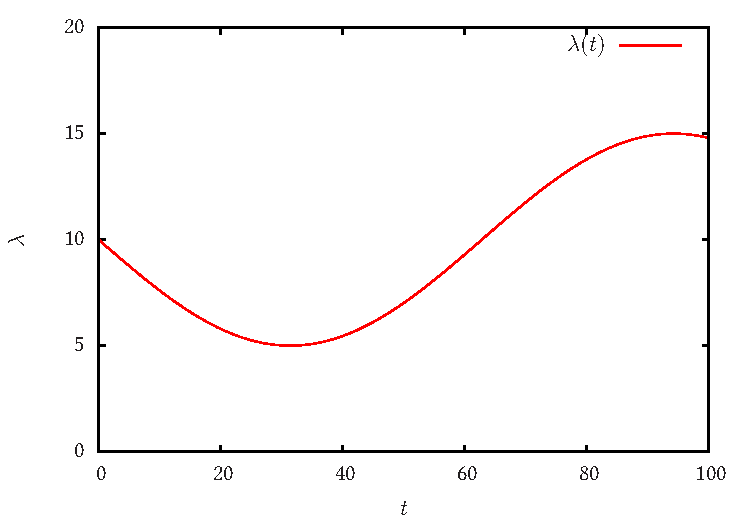
\includegraphics[width=0.5\textwidth]{prelim_sine_005}
}
\subfloat[$\alpha=0.01$]{
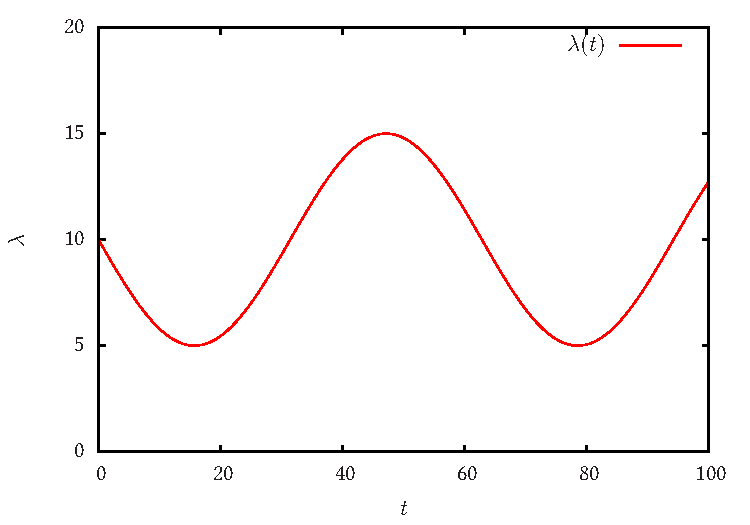
\includegraphics[width=0.5\textwidth]{prelim_sine_01}
}\\
\subfloat[$\alpha=0.015$]{
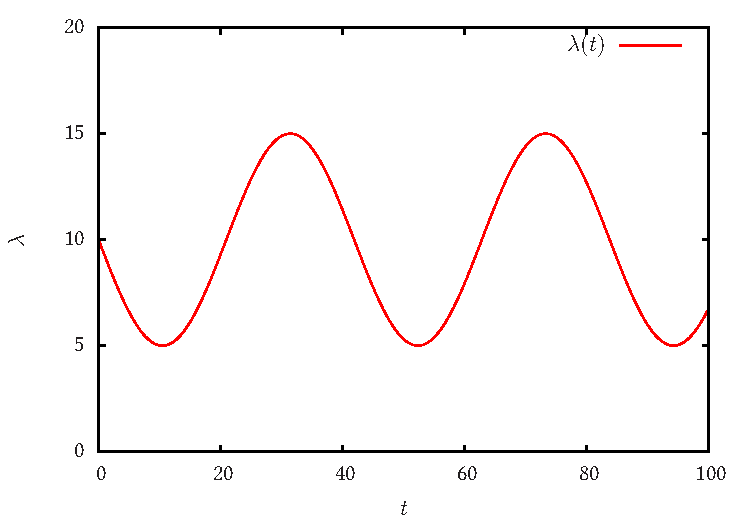
\includegraphics[width=0.5\textwidth]{prelim_sine_015}
}
\subfloat[$\alpha=0.03$]{
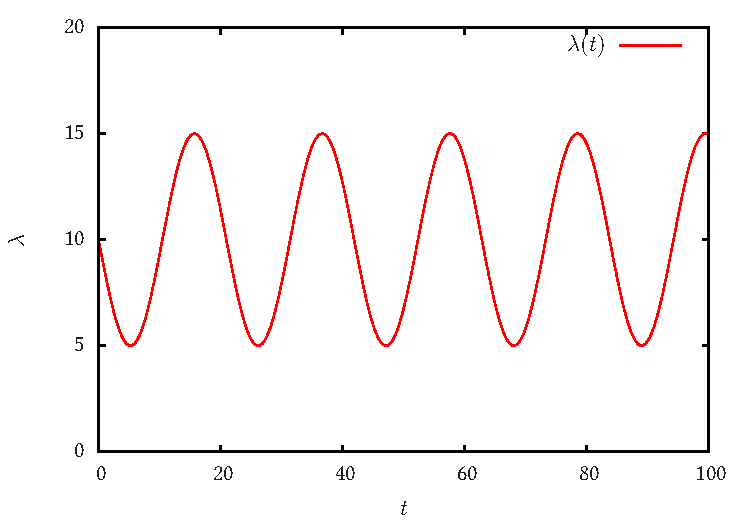
\includegraphics[width=0.5\textwidth]{prelim_sine_03}
}\\
\begin{center}
\subfloat[$\alpha=0.06$]{
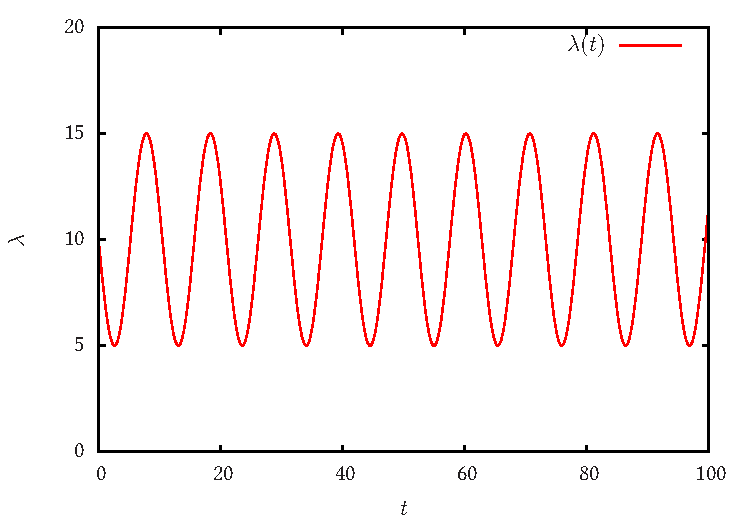
\includegraphics[width=0.5\textwidth]{prelim_sine_06}
}
\end{center}
\caption{Functions used for preliminary experiments on sine functions, showing
the different $\alpha$ values used.}
\label{fig:avals}
\end{figure}
\subsubsection{Preliminary Experiments}
\label{sec-7-1-1}

In the first set of experiments, we investigate the performance of the
estimators on five values of $\alpha$: 0.05, 0.1, 0.15, 0.3 and 0.6. Figure
\ref{fig:avals} gives an indication of what the functions look like. For
each value of $\alpha$, 25 pairs of streams were independently generated, each
with an interval of 100 time units and a time delay of 10 time steps between the
two streams. The Gaussian estimator was set to sample the kernels at a
resolution of 0.3 time steps, and the standard deviation of the kernels was
varied. The baseline estimator was set to use 3 iterations of the
IWLS estimator, and four other parameters were experimented on.
\begin{description}
\item[IWLS sub-intervals] 2, 4, 6, 8, 10
\item[PDF threshold] 0.01 to 0.15 with a step of 0.01
\item[Maximum extension] 5, 7, 9, 11, 13, 15, 17, 19, 20
\item[Maximum breakpoints] As above
\item[Gaussian standard deviation] 0.5 to 20 with a step of 0.5
\end{description}
The parameters were co-varied, meaning that each value for one
of the parameter settings was tested with all possible values of the other
parameters, for a total of 6115 possible combinations, resulting in 152,875 runs
of the function estimator for each value of $\alpha$.

Estimates appear to be reasonably accurate until $\alpha$ exceeds 0.01, after
which errors become much greater, and standard deviation increases. The area
time delay estimator is significantly better than the PDF for both of the
function estimators, with $p$-values of 0.00017 and 0.0000074 for the baseline
and Gaussian method respectively at $\alpha=$ 0.005. The difference between the
two function estimation methods was not significant, with $p$-values in excess
of 0.4 for comparisons between the baseline and Gaussian estimators for the same
time delay estimators at $\alpha=$ 0.005. Results from $\alpha>$ 0.005 show no
statistical significance in the difference between the various estimators, so
although the $p$-values at $\alpha$ =0.005 are significant, they are not
sufficient to say that the area estimator is always better. Figure
\ref{fig:prelimerror} shows the error of the various estimator combination at
each value of alpha.

\begin{table}[htb]
\caption{Experimental results for $\alpha=$ 0.005. Actual time delay is 10. ($\mu\pm\sigma$)} \label{fig:pretab}
\begin{center}
\begin{tabular}{l|ll}
       &  Gaussian           &  Baseline           \\
\hline
 Area  &  10.39 $\pm$ 3.60   &  11.43 $\pm$ 6.18   \\
 PDF   &  22.20 $\pm$ 10.94  &  22.06 $\pm$ 11.20  \\
\end{tabular}
\end{center}
\end{table}


\begin{center}
\begin{figure}
\subfloat[Baseline area]{
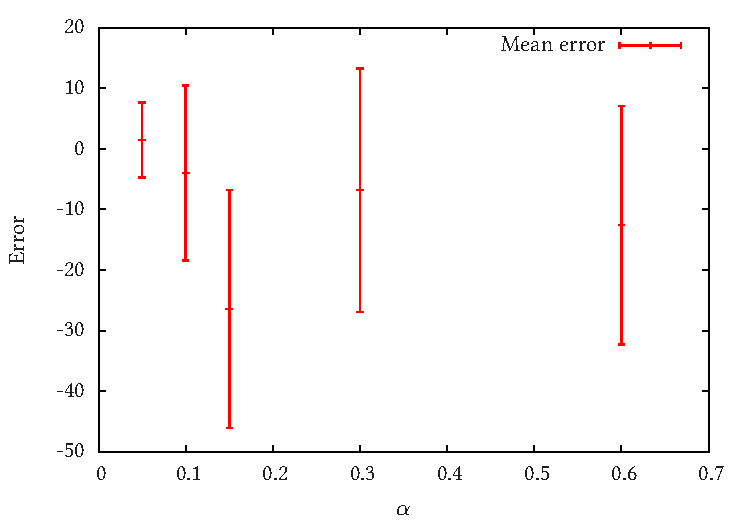
\includegraphics[width=0.5\textwidth]{base_area_prelim}
}
\subfloat[Baseline PDF]{
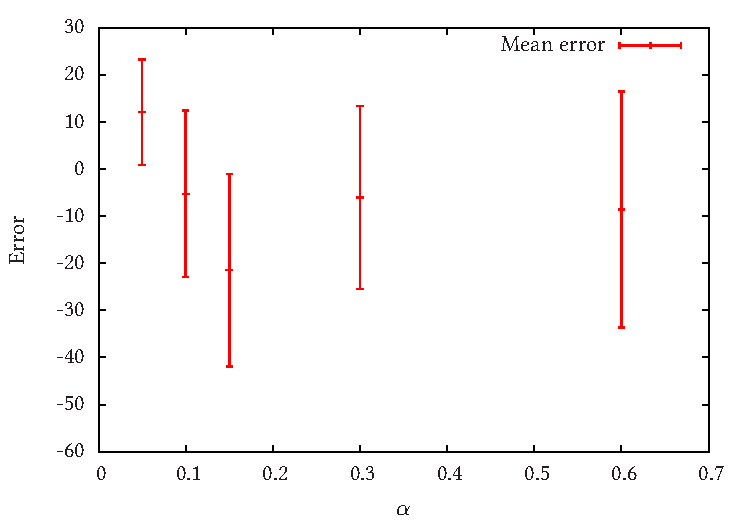
\includegraphics[width=0.5\textwidth]{base_pmf_prelim}
}\\
\subfloat[Gaussian area]{
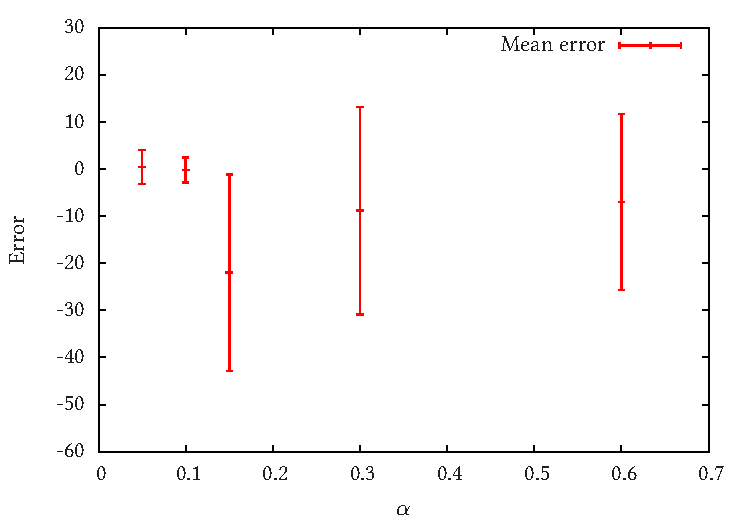
\includegraphics[width=0.5\textwidth]{gauss_area_prelim}
}
\subfloat[Gaussian PDF]{
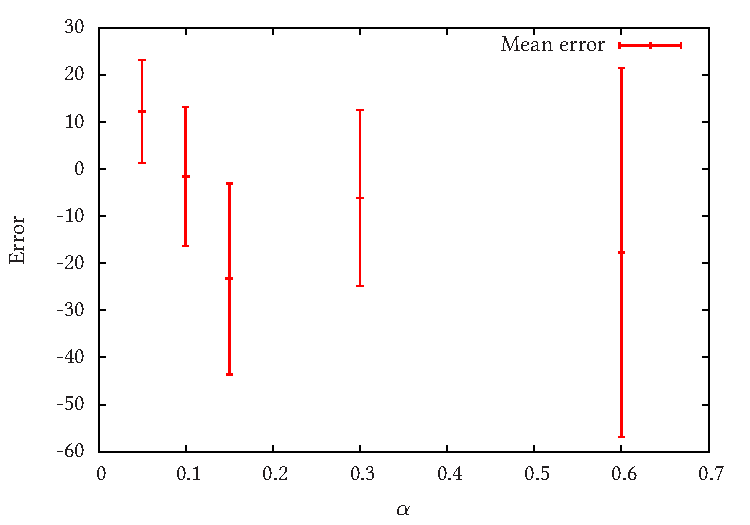
\includegraphics[width=0.5\textwidth]{gauss_pmf_prelim}
}
\caption{Error on the preliminary experiments. Error bars show standard
deviation of error. Performance appears to deteriorate when $\alpha>0.01$.}
\label{fig:prelimerror}
\end{figure}
\end{center}
\subsubsection{Refined experiments}
\label{sec-7-1-2}

Although the previous set of experiments provide some indication as to the
performance of the estimators, we investigated their effectiveness on a smaller
range of $\alpha$ values. In this set of experiments, we used the same
parameters, but generated a new set of functions for value of $\alpha$ from
0.001 to 0.015, with a step of 0.001 between each successive set of stream
pairs. For each value of $\alpha$, 10 pairs of streams were generated. The time
delay was set to 15 time steps, and the experiments were run with the same set
of experimental parameters as the previous experiments.

The result of this second set of experiments uncovered an interesting pattern in
the performance of the estimators. Figure \ref{fig:fineerror} shows the error
for each combination of estimators for different values of $\alpha$. It is clear
to see from the graphs that there is a window of optimum performance where
$\alpha$ is between 0.004 and 0.01. As with the previous set of experiments, the
area estimator again outperforms the PDF estimator, which is visible in the
graphs. Within this window, the area method is significantly better than the PDF
estimator in some cases, but this significance varies greatly as $\alpha$
varies, and we therefore cannot conclude that there is a definite increase in
accuracy using the area method. As before, the Gaussian and baseline methods do
not differ significantly in performance, but on average the Gaussian method
performs slightly better, having smaller standard deviations than the area
method.
\begin{center}
\begin{figure}
\subfloat[Baseline area]{
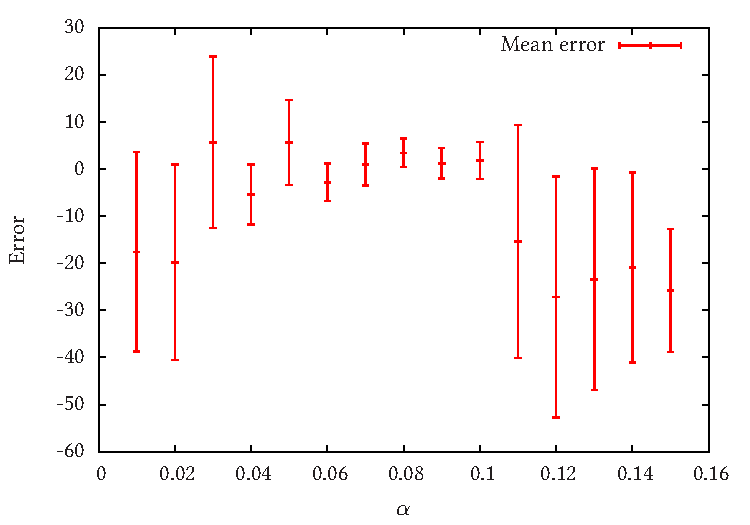
\includegraphics[width=0.5\textwidth]{baseline_area_fine}
}
\subfloat[Baseline PDF]{
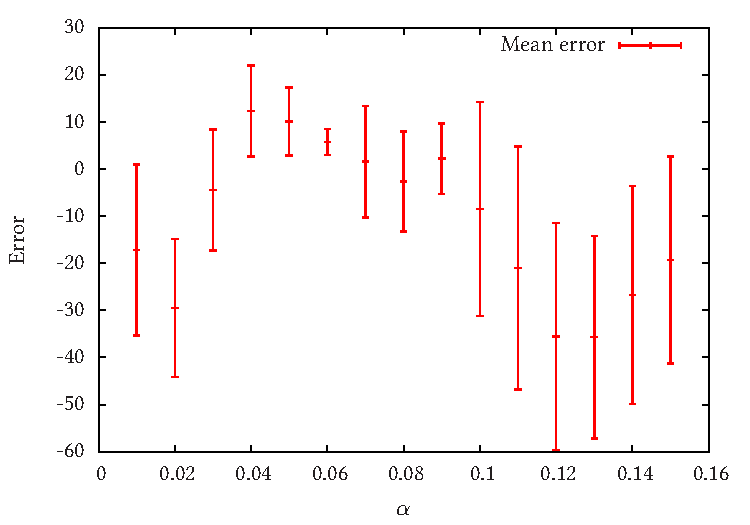
\includegraphics[width=0.5\textwidth]{baseline_pmf_fine}
}\\
\subfloat[Gaussian area]{
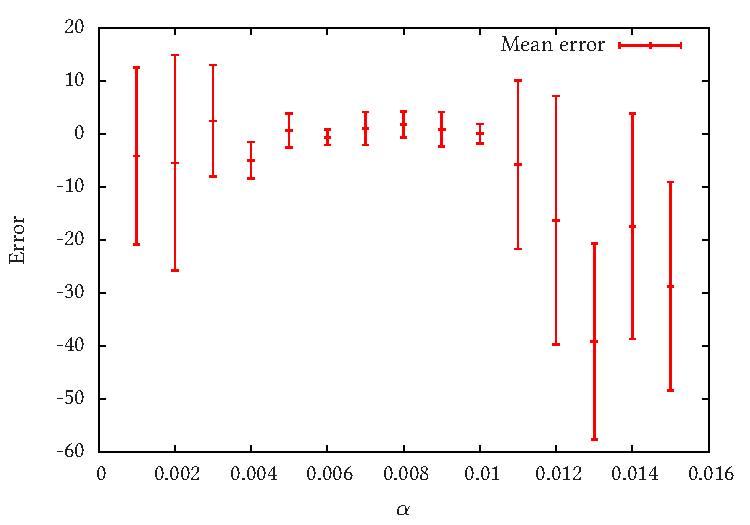
\includegraphics[width=0.5\textwidth]{gaussian_area_fine}
}
\subfloat[Gaussian PDF]{
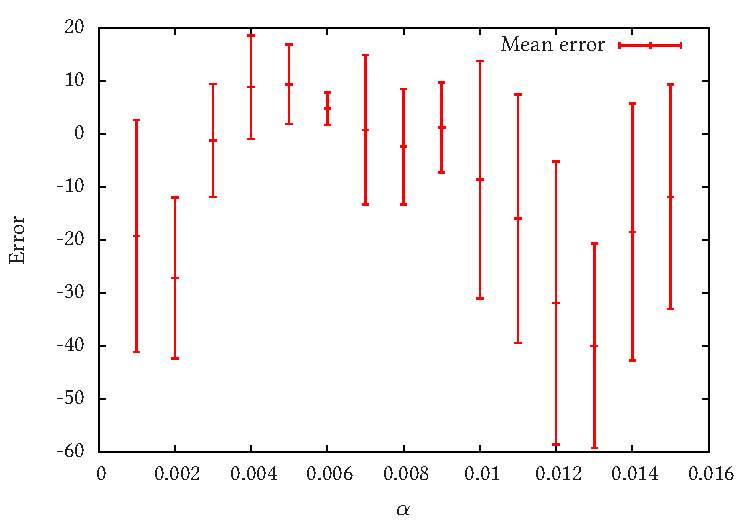
\includegraphics[width=0.5\textwidth]{gaussian_pmf_fine}
}
\caption{Error on the second set of experiments. Error bars show
standard deviation of error. Peak performance is in the window 0.004
$\leq\alpha\leq$ 0.01}
\label{fig:fineerror}
\end{figure}
\end{center}
\subsection{Random Functions}
\label{sec-7-2}

The experiments on sine functions have not yielded any definitive result as to
which methods are more effective, and so we also performed a series of
experiments using random functions rather than sine curves. Evaluating the
performance of the estimator on these functions is important, since functions
from real lensed objects will be very unlikely to follow a perfect sine curve,
instead fluctuating somewhat randomly. In order to test a variety of different
functions, vary the $\alpha$ parameter in the equation $\sigma=\alpha\cdot\Delta
t$, where $\sigma$ is the standard deviation of the Gaussians used to generate
the random function. The weight of each Gaussian was set to 3, to give a larger
range of shapes that the function could take on.
\subsubsection{Preliminary Experiment}
\label{sec-7-2-1}

For the preliminary experiment, we chose to use five different values of
$\alpha$, 0.4, 0.8, 1, 2 and 3. While increasing the $\alpha$ parameter in the
previous set of experiments would make the functions more difficult to estimate,
in this case the opposite is true; larger values are easier to estimate, whereas
smaller values are more difficult. This is due to the relationship of $\alpha$
and the standard deviation of the Gaussians used to generate the functions. For
the preliminary experiments we set the value of $\Delta t$ to be 10, resulting
in 11 Gaussians being spread uniformly across the 100 time unit interval. Given
that $\alpha$ ranges from 0.4 to 3, the value of $\sigma$ will be between 4 and
30 time units. Lower values of $\sigma$ result in each Gaussian being spread
over a smaller interval, which in turn means that when the Gaussians are summed
to construct the function it will have more variation than with large values. We
generated 5 different functions for each value of $\alpha$, and from each of
these generated 5 pairs of photon streams. In these initial experiments, we wish
to discover where the point of deterioration is, so that we can look at the
region close to this in more detail in a subsequent set of experiments. We use
the same set of experimental parameters as in the previous set of experiments:
\begin{description}
\item[IWLS sub-intervals] 2, 4, 6, 8, 10
\item[PDF threshold] 0.01 to 0.15 with a step of 0.01
\item[Maximum extension] 5, 7, 9, 11, 13, 15, 17, 19, 20
\item[Maximum breakpoints] As above
\item[Gaussian standard deviation] 0.5 to 20 with a step of 0.5
\end{description}

\begin{center}
\begin{figure}
\subfloat[$\alpha=0.4$]{
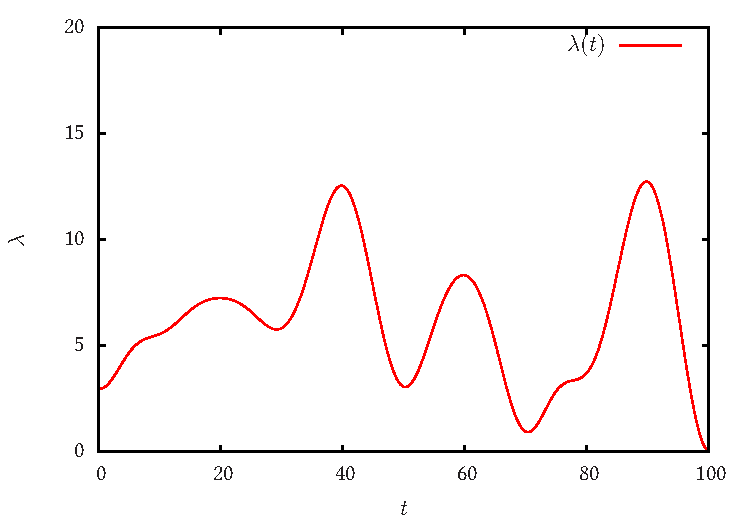
\includegraphics[width=0.5\textwidth]{randfunc_04}
}
\subfloat[$\alpha=0.8$]{
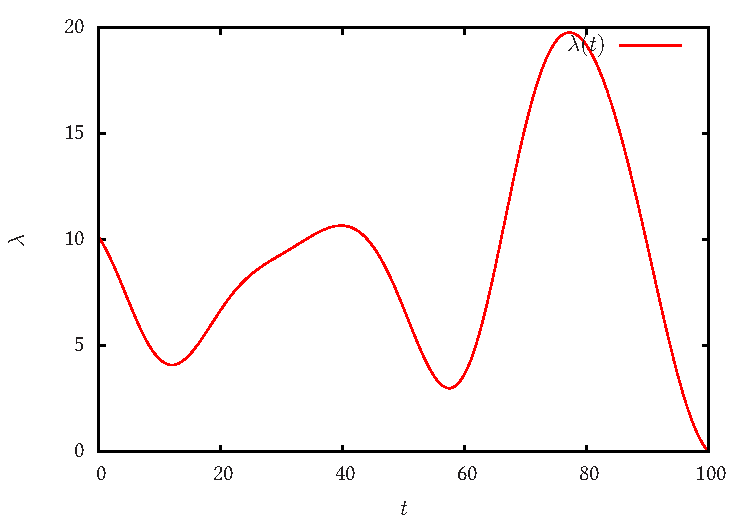
\includegraphics[width=0.5\textwidth]{randfunc_08}
}\\
\subfloat[$\alpha=1$]{
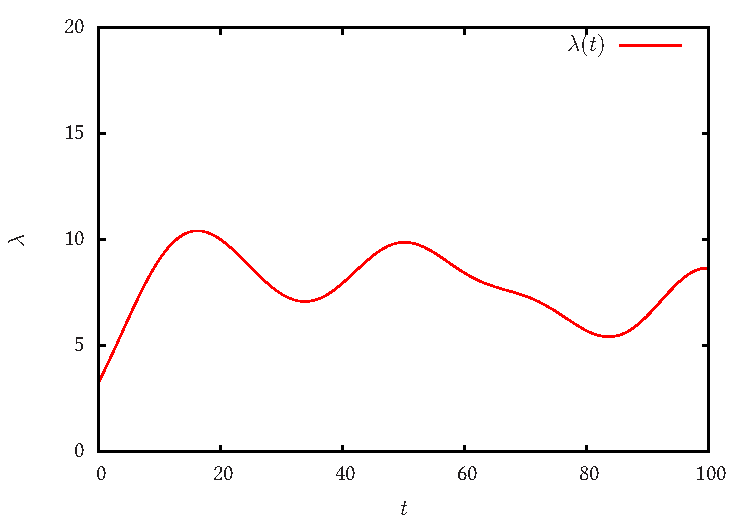
\includegraphics[width=0.5\textwidth]{randfunc_1}
}
\subfloat[$\alpha=2$]{
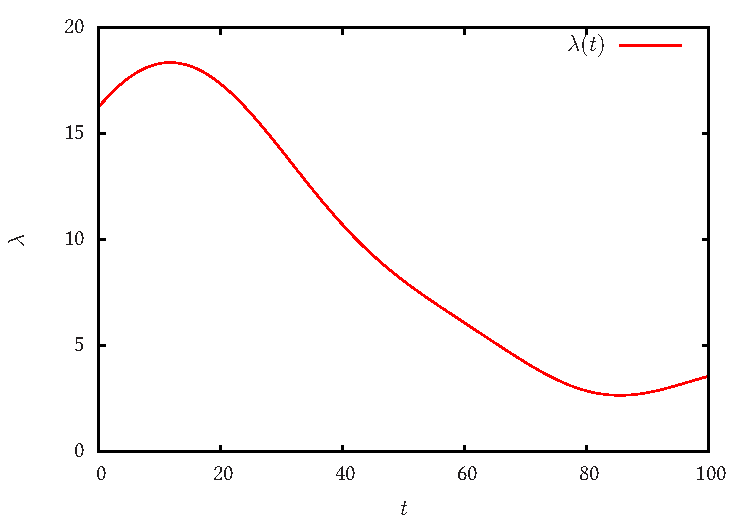
\includegraphics[width=0.5\textwidth]{randfunc_2}
}\\
\begin{center}
\subfloat[$\alpha=3$]{
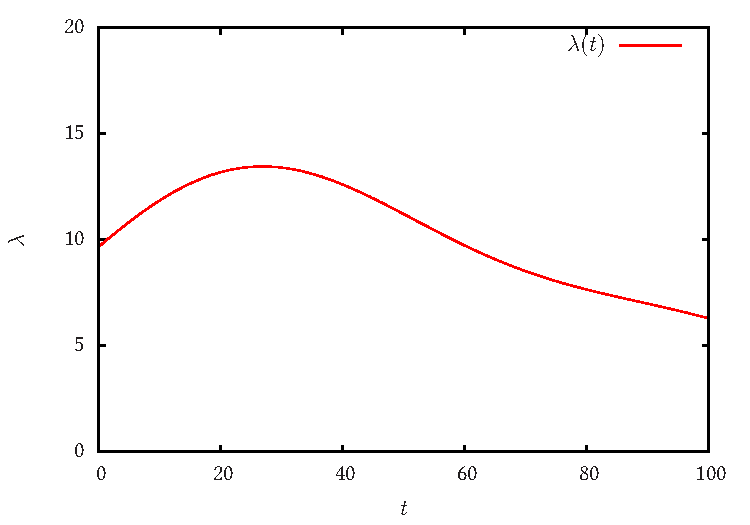
\includegraphics[width=0.5\textwidth]{randfunc_3}
}
\end{center}
\caption{Examples of random functions generated by different
values of $\alpha$. Oscillation of the functions decreases as $\alpha$ increases.}
\label{fig:randex}
\end{figure}
\end{center}
\section{Conclusion}
\label{sec-8}
\subsection{Future Work and Improvements}
\label{sec-8-1}

\begin{itemize}
\item Poisson generator - must set lambda to be greater than the value of the
  function at all points, otherwise it breaks. There are some methods of fixing this
\item baseline estimator - better way of joining functions - use the pmf to
  calculate the best possible point at which to join all points on the
  estimates. Use a hierarchical method to scan across the points between the
  points on the y axis and find the best values for all breakpoints
\end{itemize}
\subsection{Individual Comments}
\label{sec-8-2}

\begin{itemize}
\item using random libraries which are not very well documented
\item using a language that I did not know before starting
\item Working in an area that I did not know before, which required quite a lot of
  mathematical understanding
\item Working with a large system, and having to work to specific goals
\item learning from mistakes(?)
\end{itemize}

\newpage
\printbibliography
\newpage
\begin{appendices}
\section{Installation}
\label{sec-9}
\subsection{MuParser}
\label{sec-9-1}

 download package\\
 run \texttt{./configure --prefix=/usr}, followed by \texttt{make \&\& make install} (may require sudo)
 this installs muparser so that headers can be found in \texttt{/usr/include}
 \begin{verbatimtab}   
 sudo apt-get install libgsl0-dev check 
 \end{verbatimtab}
\section{Usage}
\label{sec-10}
\subsection{Creating functions for experimentation}
\label{sec-10-1}

   Generate 10 random functions using gaussians, and output the transforms as
   well so they can be plotted
   \begin{verbatimtab}
   ./launcher -g ../data/params.txt -r -t 2 -c 10
   \end{verbatimtab}
   Generate two streams from each of these generated functions using the
   gaussian generator
   \begin{verbatimtab}
   ./launcher -g ../data/params.txt -f rand -n 2 -c 10
   \end{verbatimtab}
   Generate stuttered streams from files in this directory, so that you can
   perform model fitting to find the best parameters to use on the generated
   set.
   \begin{verbatimtab}
   ./launcher -x ../data/exp_params.txt -p ../data/params.txt -c 10 -n 2 -s -i .
   \end{verbatimtab}
\section{Experimental Data}
\label{sec-11}

In this appendix we present the full set of experimental data. BA=baseline area,
GA=Gaussian area, BP=baseline PDF, GP=Gaussian PDF. BA/GA indicates a test
comparing the Gaussian area method against the baseline area method.
\begin{table}[htb]
\caption{Table of mean estimate and standard deviation for the area estimator on the first set of sine experiments ($\mu\pm\sigma$). The actual time delay is 10.} 
\begin{center}
\begin{tabular}{r|ll}
 $\alpha$  &  Baseline area               &  Gaussian area               \\
\hline
    0.005  &  11.432000 $\pm$ 6.180791    &  10.388000 $\pm$ 3.603367    \\
     0.01  &  6.008000 $\pm$ 14.456470    &  9.760000 $\pm$ 2.665033     \\
    0.015  &  -16.440000 $\pm$ 19.618053  &  -12.024000 $\pm$ 20.848622  \\
     0.03  &  3.152000 $\pm$ 20.093902    &  1.140000 $\pm$ 22.006308    \\
     0.06  &  -2.620000 $\pm$ 19.709754   &  3.000000 $\pm$ 18.653279    \\
\end{tabular}
\end{center}
\end{table}


\begin{table}[htb]
\caption{Table of mean estimate and standard deviation for the PDF estimator on the first set of sine experiments ($\mu\pm\sigma$). The actual time delay is 10.} 
\begin{center}
\begin{tabular}{r|ll}
 $\alpha$  &  Baseline PDF                &  Gaussian PDF                \\
\hline
    0.005  &  22.064000 $\pm$ 11.200353   &  22.200000 $\pm$ 10.936178   \\
     0.01  &  4.712000 $\pm$ 17.676545    &  8.420000 $\pm$ 14.729481    \\
    0.015  &  -11.472000 $\pm$ 20.411242  &  -13.308000 $\pm$ 20.256197  \\
     0.03  &  3.940000 $\pm$ 19.404082    &  3.840000 $\pm$ 18.671454    \\
     0.06  &  1.404000 $\pm$ 25.021902    &  -7.744000 $\pm$ 39.142571   \\
\end{tabular}
\end{center}
\end{table}



\begin{table}[htb]
\caption{Table of paired t-test $p$-values for preliminary sine experiments} 
\begin{center}
\begin{tabular}{r|rrrrrr}
 $\alpha$  &    BA/GA  &       BA/BP  &       BA/GP  &        GA/BP  &          GA/GP  &    BP/GP  \\
\hline
    0.005  &  0.47815  &  0.00017369  &  0.00011531  &  0.000012894  &  0.000007.3895  &  0.96623  \\
    0.010  &  0.21721  &     0.78218  &     0.56963  &      0.17294  &        0.66295  &  0.43371  \\
    0.015  &  0.45352  &     0.39424  &     0.58888  &      0.92654  &        0.82960  &  0.75580  \\
    0.030  &  0.74226  &     0.89066  &     0.90272  &      0.64223  &        0.64879  &  0.98556  \\
    0.060  &  0.31540  &     0.53891  &     0.56946  &      0.80325  &        0.23073  &  0.33954  \\
\end{tabular}
\end{center}
\end{table}


\begin{table}[htb]
\caption{Table of $p$-values for preliminary sine experiments for one sample t-test performed on error values} 
\begin{center}
\begin{tabular}{r|rrrrrr}
 $\alpha$  &    BA/GA  &        BA/BP  &        BA/GP  &         GA/BP  &         GA/GP  &    BP/GP  \\
\hline
    0.005  &  0.40134  &  0.000034334  &  0.000027901  &  0.0000037237  &  0.0000045120  &  0.87340  \\
    0.010  &  0.19016  &      0.77691  &      0.58516  &       0.16046  &       0.65594  &  0.35306  \\
    0.015  &  0.44337  &      0.39762  &      0.54968  &       0.92600  &       0.84756  &  0.72240  \\
    0.030  &  0.77304  &      0.90010  &      0.89556  &       0.60185  &       0.54686  &  0.98399  \\
    0.060  &  0.25471  &      0.49996  &      0.56251  &       0.75755  &       0.22830  &  0.27032  \\
\end{tabular}
\end{center}
\end{table}


\begin{table}[htb]
\caption{Table of mean estimate and standard deviation for the area estimator on the second set of sine experiments ($\mu\pm\sigma$). The actual time delay is 15.} 
\begin{center}
\begin{tabular}{r|ll}
 $\alpha$  &  Baseline area               &  Gaussian area               \\
\hline
    0.001  &  -2.600000 $\pm$ 21.170876   &  10.810000 $\pm$ 16.690983   \\
    0.002  &  -4.800000 $\pm$ 20.772193   &  9.490000 $\pm$ 20.362635    \\
    0.003  &  20.670000 $\pm$ 18.167171   &  17.410000 $\pm$ 10.515365   \\
    0.004  &  9.580000 $\pm$ 6.362515     &  9.970000 $\pm$ 3.435127     \\
    0.005  &  20.580000 $\pm$ 9.031810    &  15.610000 $\pm$ 3.206384    \\
    0.006  &  12.170000 $\pm$ 3.972417    &  14.300000 $\pm$ 1.483914    \\
    0.007  &  15.950000 $\pm$ 4.505164    &  15.990000 $\pm$ 3.094657    \\
    0.008  &  18.420000 $\pm$ 3.027144    &  16.700000 $\pm$ 2.463331    \\
    0.009  &  16.190000 $\pm$ 3.238657    &  15.830000 $\pm$ 3.249323    \\
    0.010  &  16.790000 $\pm$ 3.952075    &  15.010000 $\pm$ 1.823431    \\
    0.011  &  -0.360000 $\pm$ 24.729586   &  9.130000 $\pm$ 15.919991    \\
    0.012  &  -12.190000 $\pm$ 25.523105  &  -1.360000 $\pm$ 23.433745   \\
    0.013  &  -8.420000 $\pm$ 23.478705   &  -24.210000 $\pm$ 18.468701  \\
    0.014  &  -5.960000 $\pm$ 20.159623   &  -2.490000 $\pm$ 21.265674   \\
    0.015  &  -10.830000 $\pm$ 13.065301  &  -13.800000 $\pm$ 19.642301  \\
\end{tabular}
\end{center}
\end{table}


\begin{table}[htb]
\caption{Table of mean estimate and standard deviation for the PDF estimator on the second set of sine experiments ($\mu\pm\sigma$). The actual time delay is 15.} 
\begin{center}
\begin{tabular}{r|ll}
 $\alpha$  &  Baseline PDF                &  Gaussian PDF                \\
\hline
    0.001  &  -2.210000 $\pm$ 18.145603   &  -4.320000 $\pm$ 21.909030   \\
    0.002  &  -14.510000 $\pm$ 14.649877  &  -12.220000 $\pm$ 15.201368  \\
    0.003  &  10.490000 $\pm$ 12.841686   &  13.720000 $\pm$ 10.651742   \\
    0.004  &  27.300000 $\pm$ 9.604582    &  23.750000 $\pm$ 9.770491    \\
    0.005  &  25.060000 $\pm$ 7.197249    &  24.300000 $\pm$ 7.483983    \\
    0.006  &  20.720000 $\pm$ 2.740365    &  19.710000 $\pm$ 3.088187    \\
    0.007  &  16.530000 $\pm$ 11.795258   &  15.720000 $\pm$ 14.064267   \\
    0.008  &  12.350000 $\pm$ 10.595589   &  12.520000 $\pm$ 10.929026   \\
    0.009  &  17.160000 $\pm$ 7.496693    &  16.170000 $\pm$ 8.510823    \\
    0.010  &  6.480000 $\pm$ 22.690914    &  6.310000 $\pm$ 22.376168    \\
    0.011  &  -6.030000 $\pm$ 25.816934   &  -1.060000 $\pm$ 23.423373   \\
    0.012  &  -20.620000 $\pm$ 24.161945  &  -16.970000 $\pm$ 26.655433  \\
    0.013  &  -20.710000 $\pm$ 21.445766  &  -25.040000 $\pm$ 19.282334  \\
    0.014  &  -11.750000 $\pm$ 23.115720  &  -3.530000 $\pm$ 24.266275   \\
    0.015  &  -4.360000 $\pm$ 21.956102   &  3.070000 $\pm$ 21.171776    \\
\end{tabular}
\end{center}
\end{table}


\begin{table}[htb]
\caption{Table of paired t-test $p$-values for second set of sine experiments.} 
\begin{center}
\begin{tabular}{r|rrrrrr}
 $\alpha$  &      BA/GA  &       BA/BP  &       BA/GP  &         GA/BP  &       GA/GP  &      BP/GP  \\
\hline
    0.001  &    0.15295  &     0.96699  &     0.86740  &       0.13054  &     0.11670  &    0.82642  \\
    0.002  &   0.157811  &    0.266797  &    0.398533  &      0.010178  &    0.019558  &   0.748621  \\
    0.003  &    0.64686  &     0.18670  &     0.33527  &       0.22703  &     0.46908  &    0.56859  \\
    0.004  &    0.87326  &   0.0002154  &   0.0018482  &   0.000075319  &  0.00085570  &    0.44706  \\
    0.005  &  0.1371851  &   0.2597158  &   0.3539836  &     0.0020559  &   0.0049413  &  0.8286646  \\
    0.006  &    0.14919  &  0.00004719  &  0.00027971  &  0.0000078065  &  0.00016456  &    0.47247  \\
    0.007  &    0.98273  &     0.89192  &     0.96325  &       0.89579  &     0.95576  &    0.89615  \\
    0.008  &    0.20268  &     0.11576  &     0.13599  &       0.24583  &     0.27772  &    0.97364  \\
    0.009  &    0.81655  &     0.72573  &     0.99482  &       0.63121  &     0.91209  &    0.79640  \\
    0.010  &    0.23567  &     0.19600  &     0.18339  &       0.27572  &     0.26019  &    0.98741  \\
    0.011  &    0.34587  &     0.63994  &     0.95152  &       0.15109  &     0.29466  &    0.67393  \\
    0.012  &    0.36082  &     0.48103  &     0.70215  &       0.10321  &     0.20355  &    0.76434  \\
    0.013  &    0.13020  &     0.26141  &     0.11813  &       0.71497  &     0.92673  &    0.65779  \\
    0.014  &    0.72652  &     0.57817  &     0.81986  &       0.38812  &     0.92404  &    0.47133  \\
    0.015  &   0.710077  &    0.457267  &    0.110994  &      0.349136  &    0.096720  &   0.474311  \\
\end{tabular}
\end{center}
\end{table}


\begin{table}[htb]
\caption{Table of $p$-values for second set of sine experiments for one-sample t-test performed on error values} 
\begin{center}
\begin{tabular}{r|rrrrrr}
 $\alpha$  &     BA/GA  &        BA/BP  &       BA/GP  &        GA/BP  &       GA/GP  &     BP/GP  \\
\hline
    0.001  &  0.238363  &     0.963181  &    0.834164  &     0.109943  &    0.083662  &  0.718245  \\
    0.002  &  0.012781  &     0.337071  &    0.318196  &     0.020011  &    0.011247  &  0.693379  \\
    0.003  &   0.70689  &      0.28411  &     0.42725  &      0.17888  &     0.27976  &   0.46476  \\
    0.004  &   0.85129  &  0.000056159  &   0.0016052  &  0.000071618  &  0.00051425  &   0.11740  \\
    0.005  &   0.13016  &      0.29164  &     0.38843  &   0.00076639  &   0.0017663  &   0.20065  \\
    0.006  &   0.12141  &   0.00027185  &  0.00054176  &  0.000034371  &  0.00034019  &  0.058177  \\
    0.007  &   0.96101  &      0.89812  &     0.96606  &      0.89112  &     0.95491  &   0.65016  \\
    0.008  &  0.093847  &     0.128048  &    0.147634  &     0.223662  &    0.252733  &  0.634744  \\
    0.009  &   0.71169  &      0.73272  &     0.99485  &      0.66951  &     0.91808  &   0.36155  \\
    0.010  &   0.28488  &      0.22685  &     0.21387  &      0.29118  &     0.27635  &   0.66831  \\
    0.011  &   0.23385  &      0.66956  &     0.95495  &      0.10105  &     0.18555  &   0.61964  \\
    0.012  &   0.42867  &      0.60176  &     0.75116  &      0.11260  &     0.20142  &   0.67466  \\
    0.013  &   0.16087  &      0.33354  &     0.14625  &      0.48521  &     0.91090  &   0.37568  \\
    0.014  &   0.74527  &      0.64935  &     0.84987  &      0.33823  &     0.91812  &   0.15872  \\
    0.015  &   0.74025  &      0.52892  &     0.17196  &      0.40520  &     0.18736  &   0.39848  \\
\end{tabular}
\end{center}
\end{table}



\begin{table}
\subfloat[]{
\begin{tabular}{l|ll}
       &  Baseline             &  Gaussian             \\
\hline
 Area  &  17.884 $\pm$ 6.7225  &  16.62 $\pm$ 1.9959   \\
 PDF   &  13.096 $\pm$ 10.82   &  15.132 $\pm$ 11.392  \\
\end{tabular}
}
\subfloat[]{
\begin{tabular}{l|ll}
       &  Baseline             &  Gaussian             \\
\hline
 Area  &  16.472 $\pm$ 4.6097  &  15.424 $\pm$ 1.5155  \\
 PDF   &  15.64 $\pm$ 4.566    &  15.644 $\pm$ 0.6141  \\
\end{tabular}
}\\
\subfloat[]{
\begin{tabular}{l|ll}
       &  Baseline             &  Gaussian             \\
\hline
 Area  &  7.216 $\pm$ 18.96    &  13.6 $\pm$ 8.0519    \\
 PDF   &  15.156 $\pm$ 8.9448  &  13.056 $\pm$ 9.1612  \\
\end{tabular}
}
\subfloat[]{
\begin{tabular}{l|ll}
       &  Baseline             &  Gaussian             \\
\hline
 Area  &  15.068 $\pm$ 0.6497  &  14.932 $\pm$ 0.9018  \\
 PDF   &  15.052 $\pm$ 3.0461  &  14.62 $\pm$ 4.2005   \\
\end{tabular}
}\\
\begin{center}
\subfloat[]{
\begin{tabular}{l|ll}
       &  Baseline              &  Gaussian             \\
\hline
 Area  &  16.148 $\pm$ 0.99434  &  14.844 $\pm$ 0.7548  \\
 PDF   &  15.724 $\pm$ 5.9319   &  14.176 $\pm$ 6.8956  \\
\end{tabular}
}
\end{center}
\caption{Results for preliminary random function experiments. Mean estimates
over five functions were averaged for each $\alpha$ value, and the standard
deviation was calculated from the mean values. ($\mu\pm\sigma$)}
\end{table}

\end{appendices}

\end{document}